\chapter{Численные методы}\label{ch:methods}

\section{Вычислительный код Nek500}\label{sec:ch1/nek5000}

В данной главе обсуждаются теория и численные алгоритмы решения уравнений в 
вычислительном пакете Nek5000 \textbf{ССЫЛКА}. 
%
Nek5000 это открытый код, основанный на методе спектральных элементов, разрабатываемый
уже на протяжении более 35 лет.
%
Код стал популярен среди исследователей во всем мире, в основном из-за высокой точности решения уравнений 
в сравнении с другими распространенными пакетами и возможностью паралелльных вычислений 
на большом количестве ядер.
%
\section{Метод спектральных элементов и дискретные операторы}

%
\subsection{Метод Галеркина}
%
Метод основан на постановке задачи в ее вариационной (слабой) форме, которая
эквивалентна ее интегральной форме.
%
Рассмотрим уравнение адвекции-диффузии в качестве примера: выраженное в сильной форме как
%
\begin{equation}
    \frac{\partial u}{\partial t} + c \frac{\partial u}{\partial x} = 
    \nu \frac{\partial^2 u}{\partial x^2}
\end{equation}
%

Невязка может быть определена как:
%
\begin{equation}
    L(u)= \frac{\partial u}{\partial t} + c \frac{\partial u}{\partial x} 
    - \nu \frac{\partial^2 u}{\partial x^2}
\end{equation}
%
Слабая форма получается путем умножения невязки на \textbf{тестовую функцию} $v(x)$ 
и интегрирования по области:
%
\begin{equation}
    (v,L(u))= \int_\Omega v(\frac{\partial u}{\partial t} 
    + c \frac{\partial u}{\partial x} - \nu \frac{\partial^2 u}{\partial x^2})dx = 0.
\end{equation}
%
Порядок второй производной в диффузионном слагаемом может быть понижен 
интегрированием по частям и выбором $v(x)$ такой, чтобы ее значение
было равно нулю на границе области $\partial \Omega$:
\begin{equation}\label{galerkin}
    \int_\Omega (v\frac{\partial u}{\partial t} + cv \frac{\partial u}{\partial x} 
    + \nu \frac{\partial v}{\partial x} \frac{\partial u}{\partial x})dx = 0.
\end{equation}
%
Задача в формулировки Галеркина теперь звучит так: нужно найти $u(x,t)$ такую, 
что выполняется уравнение (\ref{galerkin}).
%
Потенциальный кандидат на такое решение может быть представлен как комбинация некоторых 
\textbf{пробных функций} $\psi(x)$ так, что:
%
\begin{equation}\label{galerkin2}
    u_N(x,t) = \sum_{n=0}^N u_n(t) \psi_n(x) = \underline{\psi}(x)^T \cdot \underline{u}(t),
\end{equation}
%
где $\underline{\psi}(x)$ и $\underline{u}$ -- вектор-столбы для базисных функций и коэффициентов,
соответственно.
%
В методе Галеркина тестовая функция $v(x)$ также может быть представлена как сумма пробных функций.
%
\begin{equation}\label{galerkin3}
    v(x) = \sum_{n=0}^N v_n \psi_n(x) = \underline{\psi}(x)^T \cdot \underline{v}.
\end{equation}
%
Применяя это к слабой формулировки уравнения адвекции-диффузии и полагая для простоты $c=\nu=1$, получаем:
%
\begin{equation}\label{galerkin4}
    \sum_{i=0}^N \sum_{j=0}^N v_i (\int_\Omega \psi_i \psi_j dx) \frac{du_j}{dt} +
    \sum_{i=0}^N \sum_{j=0}^N v_i (\int_\Omega \psi^\prime_i \psi^\prime_j dx) u_j +
    \sum_{i=0}^N \sum_{j=0}^N v_i (\int_\Omega \psi_i \psi^\prime_j dx) u_j = 0,
\end{equation}
%
где символом $^\prime$ обозначена производная по $x$.
%
Это уравнение можно также переписать в матричном виде:
%
\begin{equation}\label{galerkin_matrix}
    v^T M \frac{d\underline{u}}{dt} = -v^T K \underline{u} - v^TC\underline{u},
\end{equation}
%
где
%
\begin{equation}\label{galerkin_matrix2}
    M[i,j] = \int_\Omega \psi_i(x) \psi_j(x) dx,
\end{equation}
%
\begin{equation}\label{galerkin_matrix3}
    K[i,j] = \int_\Omega  \frac{d \psi_i(x)}{dx} \frac{\psi_j(x)}{dx} dx,
\end{equation}
%
\begin{equation}\label{galerkin_matrix4}
    C[i,j] = \int_\Omega \psi_i(x) \frac{\psi_j(x)}{dx} dx,
\end{equation}
%
где $M$,$K$ и $C$ -- это матрицы массы, жесткости и конвекции, соответственно.
%
При всем этом все еще остается открытым вопрос: какие функции нужно использоваться в качетсве базисных?

\subsection{Базисные функции в методе спектральных элементов}
%
В Nek5000 используются как модальные, так и узловые базисы, основанные на методе спектральных элементов.
%
В модальном подходе выбранные базисные функции известны, а коэффициенты разложения должны быть вычислены. 
%
В узловом подходе коэффициенты являются просто узловыми значениями заданной функции, в то время как полиномиальный базис должен быть построен. 
%
Каждый подход обладает различными преимуществами или свойствами, которые могут быть использованы.
%
\subsubsection{Полиномы Лежандра (модальный базис)}
%
Многочлен Лежандра порядка $k$, обозначаемый как $L_k(x)$, является собственным решением дифференциального уравнения Лежандра, которое представлено ниже:
\begin{equation*}
-\frac{d}{dx}((1-x^2)\frac{d}{dx}L_k(x)) = k(k+1)L_k(x)
\end{equation*}
%
Многочлены Лежандра могут быть определены разными способами, и различные определения выделяют разные аспекты, 
а также указывают на связи с различными математическими структурами и физическими и численными приложениями. 
%
В физике дифференциальное уравнение Лежандра возникает естественным образом, 
когда решается уравнение Лапласа методом разделения переменных в сферических координатах.
%
Пример первых шести полиномов Лежандра показан на Рис. \ref{fig:pols} 
\begin{figure}[ht]
    \centerfloat{
        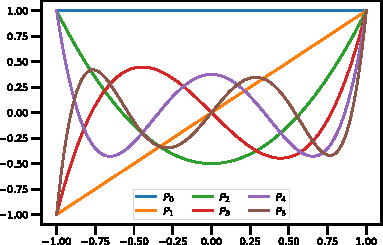
\includegraphics[scale=2.0]{legendre.pdf}
    }
    \caption{Первые шесть полиномов Лежандра.}\label{fig:pols}
\end{figure}

%
Полиномы Лежандра обладают следующими свойствами:
\begin{itemize}
    \item Ортогональность: набор многочленов Лежандра образует ортогональную систему, что означает:

    \begin{equation*}
        \int_{-1}^{1} L_m(x)L_n(x)dx = \frac{2}{2n+1}\delta_{mn}
    \end{equation*}
        
    \item Полнота: многочлены Лежандра являются полными. Это означает, что заданная кусочно-непрерывная функция $f(x)$ с конечным числом разрывов на интервале $[-1,1]$ может быть приближена следующей суммой:

    \begin{equation*}
        f_n(x) = \sum_{l=0}^{n} a_l L_l(x),
    \end{equation*}
    %
    где $a_l$ -- это коэффициент, $L_l(x)$ -- полином Лежандра степени $l$ и $f_n(x)~\rightarrow~f(x)$ при $n~\rightarrow~\infty$
    %
    Свойство полноты может быть записано в следующей форме:
    \begin{equation*}
        \sum_{l=0}^{\infty} \frac{2l+1}{2} L_l(x)L_l(y) = \delta(x-y).
    \end{equation*}
    При $x,y \in [-1,1]$ и $\delta(x-y)=\frac{1}{2\pi}\int_{-\infty}^{\infty} e^{ip(x-y)dp}$

    \item Рекуррентная формула Бонне: Многочлены Лежандра также могут быть определены как коэффициенты формального разложения в степенях $t$ производящей функции, описанной в работе Абрамовица [1974].
    \begin{equation*}
        \frac{1}{\sqrt{1-2xt+t^2}} = \sum_{n=0}^{\infty} L_n(x)t^n.
    \end{equation*}
    %
    Путем дифференцирования производящей функции по $t$ получается следующее:
    \begin{equation*}
        \frac{x-t}{\sqrt{1-2xt+t^2}} = (1-2xt+t^2)\sum_{n=1}^{\infty} nL_n(x)t^{n-1}.
    \end{equation*}
    
    Заменяя знаменатель левой части вышеприведенного уравнения суммой и перегруппировав всё уравнение, мы получаем:
    %
    \begin{equation*}
        nL_n(x)t^{n-1}-(2n+1)xL_n(x)t^n+(1+n)L_n(x)t^{n+1}=0.
    \end{equation*}
    
    Приравнивая коэффициенты при одинаковых степенях $t$, получаем:
    %
    \begin{equation*}
        (1+n)L_{1+n}(x)-(2n+1)xL_n(x)+nL_{n-1}(x) = 0, n \geq 2.
    \end{equation*}

    \item Другие свойства:
    \begin{equation*}
        \begin{aligned}
        & (2n+1)L_n(x)=L'_{n+1}(x) - L'_{n-1}(x), \\
        & L_n(-x) = (-1)^nL_n(x), \\
        & L_n(1) = 1, L_n(-1) = (-1)^n.
        \end{aligned}
    \end{equation*}

\end{itemize}

\subsubsection{Интерполяционные полиномы Лагранжа (узловой базис)}

Для элементарной сетки на $\Omega$ ($\Omega := {\xi |  −1 \leq \xi \leq 1}$), состоящей из $p + 1$ узлов 
$\Xi_{p+1} := \xi_0,...,\xi_p$, интерполяционный полином Лагранжа гладкой функции $f(\xi)$ на $[-1, 1]$ 
определяется следующим образом:
%
\begin{equation*}
    I_p f(\xi) = \sum^{p}_{i=0} f(\xi_i)\pi_i(\xi), \xi \in \Omega,
\end{equation*}
%
и
%
\begin{equation*}
    \pi_i(\xi) = \prod^{p}_{j=0, i \neq j} \frac{\xi - \xi_i}{\xi_i - \xi_j}, 0 \leq i,j \leq p.
\end{equation*}

Интересным свойством, с точки зрения метода спектральных элементов, является факт, что 
если полиномы Лагранжа применяются к точкам Гаусса-Лобатто-Лежандра (GLL), 
их также можно определить следующим образом:
%
\begin{equation*}
    \pi_i(\xi) = \frac{-1}{N(N+1)} \frac{(1-\xi^2)L'_N(\xi)}{(\xi-\xi_j)L_N(\xi_j)}, 0 \leq j \leq N.
\end{equation*}
%
Иными словами, полиномы Лагранжа можно выразить через полиномы Лежандра.
%
Также стоит ометить, что полиномы Лагранжа отличны от нуля только в интервале $\Omega = [-1, 1]$ 
и обращаются в ноль за его пределами.
%


\subsection{Метод спектральных элементов в 1D}
%
В методе спектральных элементов область интегрирования $\widetilde{\Omega}$ разбивается на интервалы (элементы). 
%
В одномерном случае разбиение $(a, b) \in \widetilde{\Omega}$  с $E$ элементами, обозначаемое как $\Delta E$, 
может быть записано следующим образом:
%
\begin{equation*}
    \Delta E: a = x_0 < x_1 < ... < x_E = b
\end{equation*}
%
Везде далее точки $\xi$ будут соотвествовать GLL точкам.
%
Для удобства численного интегрирования, необходимо отобразить элемент из физической области в 
референсную область $\Omega$.

%
В одномерном случае существует простое отображение, связывающее верхнюю границу $x^e_u$ 
и нижнюю границу $x^e_l$ элемента $e$ с референсным элементом:
%
\begin{equation*}
    x^e(\xi) = \frac{1-\xi}{2}x^e_l + \frac{1+\xi}{2}x^e_u = \frac{1+\xi}{2}(x^e_u-x^e_l) + x^e_l,
\end{equation*}
%
где $(x^e_u - x^e_l)$ -- это размер элемента $h$.
%
Аналогично можно записать и обратное отображение:
%
\begin{equation*}
    \xi(x^e)=2\frac{x^e - x^e_l}{h} - 1.
\end{equation*}

\subsubsection{Формулировка метода спектральных элементов (SEM) для уравнения переноса-диффузии 
с использованием одного элемента}
%
В данном разделе решается задача переноса-диффузии внутри одного элемента. 
%
При выборе точек GLL в качестве референсной сетки и использовании узлового подхода, 
то есть использовании полиномов Лагранжа в качестве базисных функций, 
можно завершить дискретизацию уравнения переноса-диффузии:
%
\begin{equation}\label{sem:ad}
    \int_\Omega (v\frac{\partial u}{\partial t} + cv \frac{\partial u}{\partial x} 
    + \nu \frac{\partial v}{\partial x} \frac{\partial u}{\partial x})dx = 0.
\end{equation}
%

Для этой цели вспомним процесс получения матрицы жесткости, 
анализируя только диффузионный член и принимая $\nu = 1$. 
%
Начнем со следующего выражения для элемента $e$ с областью $\Omega$:
\begin{equation*}
    \int_{\Omega^e} (\frac{\partial v}{\partial x} \frac{\partial u}{\partial x})dx 
\end{equation*}
%
Есть два основных аспекта, которые следует иметь в виду:
%

\textbf{Правило дифференцирования сложной функции}

%
В уравнении (\ref{galerkin2}) было показано, что функция $u(x, t)$ может быть представлена \
комбинацией тестовых функций и соответствующих коэффициентов. 
%
Здесь связь может быть переписана в следующей форме:
%
\begin{equation*}
    u(x)|_{\Omega^e} = \sum^N_{i=0} u^e_i \pi_i(\xi), \xi \in [-1,1].
\end{equation*}
%
Поэтому, при дифференцировании функции $u$ по переменной $x$, 
важно учитывать правило дифференцирования сложной функции:
%
\begin{equation*}
    \frac{\partial u(x)}{\partial x}|_{\Omega^e} = \sum^N_{i=0} 
    u^e_i \frac{\partial \pi_i}{\partial \xi} \frac{\partial \xi}{\partial x}, \xi \in [-1,1].
\end{equation*}
%

\textbf{Изменение области интегрирования}

%
В связи с отображением, область интегрирования в слабой формулировке уравнения меняется. 
%
Следовательно, якобиан определителя должен быть введен в качестве коэффициента масштабирования, 
который в данном случае равен:
%
\begin{equation*}
    J(\xi) = \frac{\partial x}{\partial \xi} = \frac{h}{2}.
\end{equation*}
%
Подставляя введенные обозначения в диффузионный член (\ref{sem:ad}), получим:
%
\begin{equation}\label{sem:fin}
    \int_{\Omega^e} (\frac{\partial v}{\partial x} \frac{\partial y}{\partial x})dx =
    \sum^N_{i=0} \sum^N_{j=0} v^e_i (\int_{\widetilde{\Omega}} \frac{\partial \pi_i}{\partial \xi} 
    \frac{\partial \pi_j}{\partial \xi} (\frac{\partial \xi}{\partial x})^2 J(\xi) d\xi)u^e_j.
\end{equation}
%
Это приводит к форме, аналогичной показанной во втором члене формулировки метода Галеркина (\ref{galerkin4}); 
однако теперь добавляются дополнительные члены, учитывающие отображение и геометрию элемента в физической области. 
%
Для матрицы жесткости в одномерном случае геометрический член становится постоянным, так как:
%
\begin{equation}\label{sem:fact}
    (\frac{\partial \xi}{\partial x})^2 J(\xi) = (\frac{2}{h})^2 \frac{h}{2} = \frac{2}{h}.
\end{equation}
%
Подставляя (\ref{sem:fact}) в (\ref{sem:fin}) и приводя уравнение к матричному виду, получим:
%
\begin{equation}\label{sem:matrix}
    \int_{\Omega^e} (\frac{\partial v}{\partial x} \frac{\partial y}{\partial x})dx =
    (\underline{v}^e)^T K^e \underline{u}^e,
\end{equation}
%
где
%
\begin{equation*}
    K^e[i,j] = \frac{2}{h} \int_{\widetilde{\Omega}} \frac{\partial \pi_i}{\partial \xi}
    \frac{\partial \pi_j}{\partial \xi} d\xi, \widetilde{\Omega} \in [-1,1].
\end{equation*}
%
До данного момента мы предполагали, что все интегралы оцениваются аналитически. 
%
Как мы видели, в пределах каждой области элемента мы хотим оценить интегралы следующего вида:
%
\begin{equation*}
   \int^1_{-1} f(\xi) d\xi
\end{equation*}
%

Форма функции $f(\xi)$, однако, зависит от конкретной задачи, и поэтому нам нужен автоматизированный способ оценки таких интегралов. 
%
Это подразумевает использование численного интегрирования, особенно квадратурных формул.
%
Основная идея заключается в приближении интеграла конечной суммой вида:
%
%
\begin{equation*}
    \int^1_{-1} f(\xi) d\xi = \sum^{Q-1}_{i=0}\rho_i f(\xi_i) + R(f),
\end{equation*}
%
где $\rho_i$ -- это заданные веса, а $\xi_i$ представляют собой $Q$ различных точек в интервале $−1 \leq \xi_i \leq 1$, а $R(f)$ - остаток. 
%
В частности, здесь мы используем квадратуру Гаусса-Лобатто-Лежандра:
%
\begin{equation*}
\xi_i= 
\begin{dcases}
    -1,              & i=0,\\
    \xi^{1,1}_{i-1}, & i = 1,2...Q-2,\\
    1,               & i = Q-1,
\end{dcases}
\end{equation*}
%
\begin{equation*}
    \rho_i = \frac{2}{N(N+1)}\frac{1}{[L_N(\xi_i)]^2},
\end{equation*}
%
%
\begin{equation*}
    R(f) = 0 \text{если} f(\xi) \in \textbf{P}_{2Q-3}([-1,1]).
\end{equation*}
%

В приведенных выше формулах $L_Q(\xi)$ - это полином Лежандра. 
%
Нули многочлена Якоби $\xi^{\alpha,\beta}$ (здесь $\alpha = \beta = 1$, 
они являются нулями $L'_Q(\xi)$) не имеют аналитической формы и обычно эти нули табулируются. 
%
Табулирование данных может привести к ошибкам копирования, 
поэтому лучшим способом оценки нулей является использование численного алгоритма, 
такого как метод Ньютона-Рафсона. 
%
Определив нули, веса могут быть оценены с помощью этого метода.
%
Для этого генерируется полином Лежандра с помощью рекуррентных соотношений. 
%
Квадратура GLL точна, если порядок полинома-интегранда не превышает $2Q - 3$.
%

%
Затем можно численно интегрировать и дифференцировать члены таким образом, 
чтобы получить конечную форму матрицы.
%
\begin{equation*}
    K^e[i,j] = \frac{2}{h} \sum^N_{m=0} \rho_m D^{(1)}_{N,mi} D^{(1)}_{N,mj},
\end{equation*}
%
где $D_N$ - матрица дифференцирования, полученная следующим образом:
%
\begin{equation*}
    D^{(1)}_{N,ij} = \frac{d \pi_j}{d\xi}|_{\xi=\xi_i} =
    \begin{dcases}
        \frac{L_N(\xi_i)}{L_N(\xi_j)}\frac{1}{\xi_i-\xi_j},      & i \neq j,\\
        -\frac{(N+1)N}{4}, & i = j = 0,\\
        \frac{(N+1)N}{4}, & i = j = N,\\
        0,               & \text{в остальных случаях}.
    \end{dcases}
\end{equation*}
%
Следуя такой же процедуре, что и для матрицы жесткости, 
можно получить матрицы массы и переноса, с учетом того, что $\pi_i(x_j) = \delta_{ij}$:
%
\begin{equation*}
    M^e[i,j] = \frac{h}{2} \rho_i \delta{ij},
\end{equation*}
%
%
\begin{equation*}
    C^e[i,j] = \sum^N_{m=0} \rho_m \pi_{mi} D^{(1)}_{N,mj} = \rho_i D^{(1)}_{N,ij}
\end{equation*}
%
\textbf{А что насчет нелинейностей?}
%
Нелинейный член в уравнении Навье-Стокса обрабатывается аналогично постоянному конвективному члену. 
%
Для случая с нелинейным членом $u \frac{du}{dx}$ применяются те же процедуры, 
используется ортогональность базисных функций и с учетом квадратурных правил получается следующее выражение:
%
\begin{equation*}
    C^e[i,j] = \rho_i u^e_i D^{(1)}_{N,ij}
\end{equation*}

\section{Уравнения Навье-Стокса}
%
Перейдем к рассмотрению уравнений, которые решаются в вычислительном коде Nek5000.
%
Уравнения, описывающие несжимаемые течения Ньютоновской жидкости с постоянными свойствами, имеют вид:
%
\begin{equation}\label{eq:ns}
    \frac{\partial \textbf{v}}{\partial t} = - \nabla p + \nu \textbf{L}(\textbf{v}) +
    \textbf{N}(\textbf{v}) \text{в} \Omega,
\end{equation}
%
и условие несжимаемости определяется как:
%
\begin{equation}\label{eq:cont}
    Q = \nabla \cdot \textbf{v} = 0 \text{в} \Omega.
\end{equation}
%

Здесь $\textbf{v}$ -- вектор скорости, $p$ -- давление, а кинематическая вязкость обозначается $\nabla$. 
%
Линейные и нелинейные операторы в уравнениях Навье-Стокса обозначаются как $\textbf{L}$ и $\textbf{N}$ 
и определяются следующим образом:
%
\begin{equation}\label{eq:linear}
    \textbf{L} (\textbf{v}) = \nabla^2 \textbf{v} = \nabla(\nabla \cdot \textbf{v}) - 
    \nabla \times (\nabla \times \textbf{v}).
\end{equation}
%
\begin{equation}\label{eq:nonlin}
    \textbf{N} (\textbf{v}) = - \frac{1}{2}[\textbf{v} \cdot \nabla \textbf{v} + 
    \nabla (\textbf{v} \cdot \textbf{v})]. 
\end{equation}
%
Нелинейный оператор записан в кососимметричной форме, которая представляет собой 
комбинацию конвективной и консервативной форм. 
%
Обратите внимание, что кососимметричная форма не используется в Nek5000, однако 
было удобно использовать ее в конвективной формулировке. 
%
Описанные выше уравнения Навье-Стокса требуется дискретизировать как во времени, так и в пространстве. 
%
Рассмотрим на примере уравнения (\ref{eq:ns}) один проинтегрированный по времени шаг ($\Delta t$):
%
\begin{equation}\label{eq:tstep}
    \textbf{v}^{n+1} - \textbf{v}^n = - \int^{t_{n+1}}_{t_n} \nabla p dt + 
    \nu  \int^{t_{n+1}}_{t_n} \textbf{L} (\textbf{v}) dt + \int^{t_{n+1}}_{t_n} \textbf{N} (\textbf{v}) dt, 
\end{equation}
%
где индекс $n$ обозначает шаг по времени $t_n = n \Delta t$.
%
Слагаемое с давлением запишем как:
%
\begin{equation}\label{eq:pres}
    \int^{t_{n+1}}_{t_n} \nabla p dt = \Delta t \nabla \overline{p}^{n+1},
\end{equation}        
%
где $\overline{p}^{n+1}$ -- скалярное поле, обеспечивающее несжимаемость итогового поля скорости 
к концу временного шага $(n+1)$, иными словами обеспечивающее равенство нулю дивергенции скорости.
%
Нелинейный и линейный слагаемые апрроксимируются с помощью явной и неявной схемы, соответственно.
%
Первое аппроксимируется с помощью схемы Адамса-Башфорта порядка $J_e$,
второе -- порядка $J_i$:
%
\begin{equation}\label{eq:nln}
    \int^{t_{n+1}}_{t_n} \textbf{N} (\textbf{v}) dt = \Delta t \sum_{q=0}^{J_e - 1} \beta_q \textbf{N} (\textbf{v}^{n-q}) ,
\end{equation}        
%
%
\begin{equation}\label{eq:ln}
    \int^{t_{n+1}}_{t_n} \textbf{L} (\textbf{v}) dt = \Delta t \sum_{q=0}^{J_i - 1} \gamma_q \textbf{L} (\textbf{v}^{n+1-q}) ,
\end{equation}        
%
где $\beta_q$ и $\gamma_q$ -- это правильно выбранные веса для явной и неявной схемы, соответственно REF.
%
Стоит отметить, что причина выбора неявной схемы для линейного слагаемого кроется в устойчивости схемы.
%
Также следует отметить, что левая часть уравнения (\ref{eq:tstep}) является примером метода первого порядка точности, 
а для получения так называемой жестко устойчивой схемы мы используем метод более высокого порядка 
для дискретизации $\partial v/\partial t$, который можно обобщить как:
%
%
\begin{equation}\label{eq:der}
    \frac{\partial \textbf{v}}{\partial t} = \frac{\gamma_0 \textbf{v}^{n+1} - \sum_{q=0}^{J_i-1}\alpha_q \textbf{v}^{n-q} }{\Delta t}
\end{equation}        
%
где $\alpha_q$ -- это коэффициенты жестко устойчивой схемы порядка $J_i$. 
%
Что касается $\gamma_0$, то оно определяется как $\gamma_0 = \sum_{q=0}^{J_i-1} \alpha_q$.
%
Решение приведенной выше полудискретной системы (\ref{eq:tstep}) может быть получено 
путем использования дискретизации, показанной в (\ref{eq:pres})-(\ref{eq:der}), 
и разделения вычисления на три подэтапа, как это будет показано ниже.

\section{Схема Карниадакиса}
%

Широко известная как формулировка $P_n-P_n$, схема Карниадакиса не обязательно применяется только  в методе 
спектральных элементов, хотя первоначальной она была использована именно для него. 
%
По своей сути она просто разделяет давление и скорость друг от друга. 
%
Подставляя (\ref{eq:der}) и дискретизации линейного и нелинейного членов (\ref{eq:nln}-\ref{eq:ln}) 
в (\ref{eq:ns}), приходим к следующей полудискретной системе:
%
%
\begin{equation}\label{eq:sheme}
    \frac{\gamma_0 \textbf{v}^{n+1} - \sum_{q=0}^{J_i-1}\alpha_q \textbf{v}^{n-q} }{\Delta t} =
    - \nabla \overline{p}^{n+1} + \nu \sum_{q=0}^{J_i-1} \gamma_q \textbf{L}(\textbf{v}^{n+1-q}) +
    \sum_{q=0}^{J_e-1} \beta_q \textbf{N}(\textbf{v}^{n-q})
\end{equation}        
%

Для решения этой системы в схеме Карниадакиса делается три ``подшага'':
%
\begin{equation}\label{eq:ks1}
    \frac{\Hat{\textbf{v}-\sum_{q=0}^{J_i-1}\alpha_q \textbf{v}^{n-q}} }{\Delta t} = \sum_{q=0}^{J_e-1}\beta_q \textbf{N}(\textbf{v}^{n-q}) \text{ в } \Omega
\end{equation}        
%
%
\begin{equation}\label{eq:ks2} 
    \frac{\Hat{\Hat{\textbf{v}}}-\Hat{\textbf{v}}}{\Delta t} = -\nabla \overline{p}^{n+1} \text{ в } \Omega
\end{equation}        
%
%
\begin{equation}\label{eq:ks3} 
    \frac{\gamma_0 \textbf{v}^{n+1} - \Hat{\Hat{\textbf{v}}}}{\Delta t} = \nu \nabla^2 \textbf{v}^{n+1} \text{ в } \Omega
\end{equation}        
%
с граничными условиями Дирихле:
%
\begin{equation}\label{eq:ksbc} 
    \textbf{v}^{n+1} = \overrightarrow{v}_0 \text{  на } \partial \Omega
\end{equation}        
%

Однако в этой системе скорость и давление на временном шаге $n + 1$ все еще связаны. 
%
Далее используем условие несжимаемости для поля $\textbf{v}$:


% % \chapter{Оформление различных элементов}\label{ch:ch1}

% % \section{Форматирование текста}\label{sec:ch1/sec1}



% \section{Ссылки}\label{sec:ch1/sec2}

% Сошлёмся на библиографию.
% Одна ссылка: \cite[с.~54]{Sokolov}\cite[с.~36]{Gaidaenko}.
% Две ссылки: \cite{Sokolov,Gaidaenko}.
% Ссылка на собственные работы: \cite{vakbib1, confbib2}.
% Много ссылок: %\cite[с.~54]{Lermontov,Management,Borozda} % такой «фокус»
% %вызывает biblatex warning относительно опции sortcites, потому что неясно, к
% %какому источнику относится уточнение о страницах, а bibtex об этой проблеме
% %даже не предупреждает
% \cite{Lermontov, Management, Borozda, Marketing, Constitution, FamilyCode,
%     Gost.7.0.53, Razumovski, Lagkueva, Pokrovski, Methodology, Berestova,
%     Kriger}%
% \ifnumequal{\value{bibliosel}}{0}{% Примеры для bibtex8
%     \cite{Sirotko, Lukina, Encyclopedia, Nasirova}%
% }{% Примеры для biblatex через движок biber
%     \cite{Sirotko2, Lukina2, Encyclopedia2, Nasirova2}%
% }%
% .
% И~ещё немного ссылок:~\cite{Article,Book,Booklet,Conference,Inbook,Incollection,Manual,Mastersthesis,
%     Misc,Phdthesis,Proceedings,Techreport,Unpublished}
% % Следует обратить внимание, что пробел после запятой внутри \cite{}
% % обрабатывается ожидаемо, а пробел перед запятой, может вызывать проблемы при
% % обработке ссылок.
% \cite{medvedev2006jelektronnye, CEAT:CEAT581, doi:10.1080/01932691.2010.513279,
%     Gosele1999161,Li2007StressAnalysis, Shoji199895, test:eisner-sample,
%     test:eisner-sample-shorted, AB_patent_Pomerantz_1968, iofis_patent1960}%
% \ifnumequal{\value{bibliosel}}{0}{% Примеры для bibtex8
% }{% Примеры для biblatex через движок biber
%     \cite{patent2h, patent3h, patent2}%
% }%
% .

% \ifnumequal{\value{bibliosel}}{0}{% Примеры для bibtex8
% Попытка реализовать несколько ссылок на конкретные страницы
% для \texttt{bibtex} реализации библиографии:
% [\citenum{Sokolov}, с.~54; \citenum{Gaidaenko}, с.~36].
% }{% Примеры для biblatex через движок biber
% Несколько источников (мультицитата):
% % Тут специально написано по-разному тире, для демонстрации, что
% % применение специальных тире в настоящий момент в biblatex приводит к непоказу
% % "с.".
% \cites[vii--x, 5, 7]{Sokolov}[v"--~x, 25, 526]{Gaidaenko}[vii--x, 5, 7]{Techreport},
% работает только в \texttt{biblatex} реализации библиографии.
% }%

% Ссылки на собственные работы:~\cite{vakbib1, confbib1}.

% Сошлёмся на приложения: Приложение~\cref{app:A}, Приложение~\cref{app:B2}.

% Сошлёмся на формулу: формула~\cref{eq:equation1}.

% Сошлёмся на изображение: рисунок~\cref{fig:knuth}.

% Стандартной практикой является добавление к ссылкам префикса, характеризующего тип элемента.
% Это не является строгим требованием, но~позволяет лучше ориентироваться в документах большого размера.
% Например, для ссылок на~рисунки используется префикс \textit{fig},
% для ссылки на~таблицу "--- \textit{tab}.

% В таблице \cref{tab:tab_pref} приложения~\cref{app:B4} приведён список рекомендуемых
% к использованию стандартных префиксов.

% В некоторых ситуациях возникает необходимость отойти от требований ГОСТ по оформлению ссылок на
% литературу.
% В таком случае можно воспользоваться дополнительными опциями пакета \verb+biblatex+.

% Например, в ссылке на книгу~\cite{sobenin_kdv} использование опции \verb+maxnames=4+ позволяет
% вывести имена всех четырёх авторов.
% По ГОСТ имена последних трёх авторов опускаются.

% Кроме того, часто возникают проблемы с транслитерованными инициалами. Некоторые буквы русского
% алфавита по правилам транслитерации записываются двумя буквами латинского алфавита (ю-yu, ё-yo и
% т.д.).
% Такие инициалы \verb+biblatex+ будет сокращать до одной буквы, что неверно.
% Поправить его работу можно использовав опцию \verb+giveninits=false+.
% Пример использования этой опции можно видеть в ссылке~\cite{initials}.

% \section{Формулы}\label{sec:ch1/sec3}

% Благодаря пакету \textit{icomma}, \LaTeX~одинаково хорошо воспринимает
% в~качестве десятичного разделителя и запятую (\(3,1415\)), и точку (\(3.1415\)).

% \subsection{Ненумерованные одиночные формулы}\label{subsec:ch1/sec3/sub1}

% Вот так может выглядеть формула, которую необходимо вставить в~строку
% по~тексту: \(x \approx \sin x\) при \(x \to 0\).

% А вот так выглядит ненумерованная отдельностоящая формула c подстрочными
% и надстрочными индексами:
% \[
%     (x_1+x_2)^2 = x_1^2 + 2 x_1 x_2 + x_2^2
% \]

% Формула с неопределенным интегралом:
% \[
%     \int f(\alpha+x)=\sum\beta
% \]

% При использовании дробей формулы могут получаться очень высокие:
% \[
%     \frac{1}{\sqrt{2}+
%         \displaystyle\frac{1}{\sqrt{2}+
%             \displaystyle\frac{1}{\sqrt{2}+\cdots}}}
% \]

% В формулах можно использовать греческие буквы:
% %Все \original... команды заранее, ради этого примера, определены в Dissertation\userstyles.tex
% \[
%     \alpha\beta\gamma\delta\originalepsilon\epsilon\zeta\eta\theta%
%     \vartheta\iota\kappa\varkappa\lambda\mu\nu\xi\pi\varpi\rho\varrho%
%     \sigma\varsigma\tau\upsilon\originalphi\phi\chi\psi\omega\Gamma\Delta%
%     \Theta\Lambda\Xi\Pi\Sigma\Upsilon\Phi\Psi\Omega
% \]
% \[%https://texfaq.org/FAQ-boldgreek
%     \boldsymbol{\alpha\beta\gamma\delta\originalepsilon\epsilon\zeta\eta%
%         \theta\vartheta\iota\kappa\varkappa\lambda\mu\nu\xi\pi\varpi\rho%
%         \varrho\sigma\varsigma\tau\upsilon\originalphi\phi\chi\psi\omega\Gamma%
%         \Delta\Theta\Lambda\Xi\Pi\Sigma\Upsilon\Phi\Psi\Omega}
% \]

% Для добавления формул можно использовать пары \verb+$+\dots\verb+$+ и \verb+$$+\dots\verb+$$+,
% но~они считаются устаревшими.
% Лучше использовать их функциональные аналоги \verb+\(+\dots\verb+\)+ и \verb+\[+\dots\verb+\]+.

% \subsection{Ненумерованные многострочные формулы}\label{subsec:ch1/sec3/sub2}

% Вот так можно написать две формулы, не нумеруя их, чтобы знаки <<равно>> были
% строго друг под другом:
% \begin{align}
%     f_W & =  \min \left( 1, \max \left( 0, \frac{W_{soil} / W_{max}}{W_{crit}} \right)  \right), \nonumber \\
%     f_T & =  \min \left( 1, \max \left( 0, \frac{T_s / T_{melt}}{T_{crit}} \right)  \right), \nonumber
% \end{align}

% Выровнять систему ещё и по переменной \( x \) можно, используя окружение
% \verb|alignedat| из пакета \verb|amsmath|. Вот так:
% \[
% |x| = \left\{
% \begin{alignedat}{2}
%     &&x, \quad &\text{eсли } x\geqslant 0 \\
%     &-&x, \quad & \text{eсли } x<0
% \end{alignedat}
% \right.
% \]
% Здесь первый амперсанд (в исходном \LaTeX\ описании формулы) означает
% выравнивание по~левому краю, второй "--- по~\( x \), а~третий "--- по~слову
% <<если>>. Команда \verb|\quad| делает большой горизонтальный пробел.

% Ещё вариант:
% \[
%     |x|=
%     \begin{cases}
%         \phantom{-}x, \text{если } x \geqslant 0 \\
%         -x, \text{если } x<0
%     \end{cases}
% \]

% Кроме того, для  нумерованных формул \verb|alignedat| делает вертикальное
% выравнивание номера формулы по центру формулы. Например, выравнивание
% компонент вектора:
% \begin{equation}
%     \label{eq:2p3}
%     \begin{alignedat}{2}
%         {\mathbf{N}}_{o1n}^{(j)} = \,{\sin} \phi\,n\!\left(n+1\right)
%         {\sin}\theta\,
%         \pi_n\!\left({\cos} \theta\right)
%         \frac{
%         z_n^{(j)}\!\left( \rho \right)
%         }{\rho}\,
%         &{\boldsymbol{\hat{\mathrm e}}}_{r}\,+   \\
%         +\,
%         {\sin} \phi\,
%         \tau_n\!\left({\cos} \theta\right)
%         \frac{
%         \left[\rho z_n^{(j)}\!\left( \rho \right)\right]^{\prime}
%         }{\rho}\,
%         &{\boldsymbol{\hat{\mathrm e}}}_{\theta}\,+   \\
%         +\,
%         {\cos} \phi\,
%         \pi_n\!\left({\cos} \theta\right)
%         \frac{
%         \left[\rho z_n^{(j)}\!\left( \rho \right)\right]^{\prime}
%         }{\rho}\,
%         &{\boldsymbol{\hat{\mathrm e}}}_{\phi}\:.
%     \end{alignedat}
% \end{equation}

% Ещё об отступах. Иногда для лучшей <<читаемости>> формул полезно
% немного исправить стандартные интервалы \LaTeX\ с учётом логической
% структуры самой формулы. Например в формуле~\cref{eq:2p3} добавлен
% небольшой отступ \verb+\,+ между основными сомножителями, ниже
% результат применения всех вариантов отступа:
% \begin{align*}
%     \backslash!             & \quad f(x) = x^2\! +3x\! +2         \\
%     \mbox{по-умолчанию}     & \quad f(x) = x^2+3x+2               \\
%     \backslash,             & \quad f(x) = x^2\, +3x\, +2         \\
%     \backslash{:}           & \quad f(x) = x^2\: +3x\: +2         \\
%     \backslash;             & \quad f(x) = x^2\; +3x\; +2         \\
%     \backslash \mbox{space} & \quad f(x) = x^2\ +3x\ +2           \\
%     \backslash \mbox{quad}  & \quad f(x) = x^2\quad +3x\quad +2   \\
%     \backslash \mbox{qquad} & \quad f(x) = x^2\qquad +3x\qquad +2
% \end{align*}

% Можно использовать разные математические алфавиты:
% \begin{align}
%     \mathcal{ABCDEFGHIJKLMNOPQRSTUVWXYZ} \nonumber  \\
%     \mathfrak{ABCDEFGHIJKLMNOPQRSTUVWXYZ} \nonumber \\
%     \mathbb{ABCDEFGHIJKLMNOPQRSTUVWXYZ} \nonumber
% \end{align}

% Посмотрим на систему уравнений на примере аттрактора Лоренца:

% \[
% \left\{
% \begin{array}{rl}
%     \dot x = & \sigma (y-x)  \\
%     \dot y = & x (r - z) - y \\
%     \dot z = & xy - bz
% \end{array}
% \right.
% \]

% А для вёрстки матриц удобно использовать многоточия:
% \[
%     \left(
%         \begin{array}{ccc}
%             a_{11} & \ldots & a_{1n} \\
%             \vdots & \ddots & \vdots \\
%             a_{n1} & \ldots & a_{nn} \\
%         \end{array}
%     \right)
% \]

% \subsection{Нумерованные формулы}\label{subsec:ch1/sec3/sub3}

% А вот так пишется нумерованная формула:
% \begin{equation}
%     \label{eq:equation1}
%     e = \lim_{n \to \infty} \left( 1+\frac{1}{n} \right) ^n
% \end{equation}

% Нумерованных формул может быть несколько:
% \begin{equation}
%     \label{eq:equation2}
%     \lim_{n \to \infty} \sum_{k=1}^n \frac{1}{k^2} = \frac{\pi^2}{6}
% \end{equation}

% Впоследствии на формулы~\cref{eq:equation1, eq:equation2} можно ссылаться.

% Сделать так, чтобы номер формулы стоял напротив средней строки, можно,
% используя окружение \verb|multlined| (пакет \verb|mathtools|) вместо
% \verb|multline| внутри окружения \verb|equation|. Вот так:
% \begin{equation} % \tag{S} % tag - вписывает свой текст
%     \label{eq:equation3}
%     \begin{multlined}
%         1+ 2+3+4+5+6+7+\dots + \\
%         + 50+51+52+53+54+55+56+57 + \dots + \\
%         + 96+97+98+99+100=5050
%     \end{multlined}
% \end{equation}

% Уравнения~\cref{eq:subeq_1,eq:subeq_2} демонстрируют возможности
% окружения \verb|\subequations|.
% \begin{subequations}
%     \label{eq:subeq_1}
%     \begin{gather}
%         y = x^2 + 1 \label{eq:subeq_1-1} \\
%         y = 2 x^2 - x + 1 \label{eq:subeq_1-2}
%     \end{gather}
% \end{subequations}
% Ссылки на отдельные уравнения~\cref{eq:subeq_1-1,eq:subeq_1-2,eq:subeq_2-1}.
% \begin{subequations}
%     \label{eq:subeq_2}
%     \begin{align}
%         y & = x^3 + x^2 + x + 1 \label{eq:subeq_2-1} \\
%         y & = x^2
%     \end{align}
% \end{subequations}

% \subsection{Форматирование чисел и размерностей величин}\label{sec:units}

% Числа форматируются при помощи команды \verb|\num|:
% \num{5,3};
% \num{2,3e8};
% \num{12345,67890};
% \num{2,6 d4};
% \num{1+-2i};
% \num{.3e45};
% \num[exponent-base=2]{5 e64};
% \num[exponent-base=2,exponent-to-prefix]{5 e64};
% \num{1.654 x 2.34 x 3.430}
% \num{1 2 x 3 / 4}.
% Для написания последовательности чисел можно использовать команды \verb|\numlist| и \verb|\numrange|:
% \numlist{10;30;50;70}; \numrange{10}{30}.
% Значения углов можно форматировать при помощи команды \verb|\ang|:
% \ang{2.67};
% \ang{30,3};
% \ang{-1;;};
% \ang{;-2;};
% \ang{;;-3};
% \ang{300;10;1}.

% Обратите внимание, что ГОСТ запрещает использование знака <<->> для обозначения отрицательных чисел
% за исключением формул, таблиц и~рисунков.
% Вместо него следует использовать слово <<минус>>.

% Размерности можно записывать при помощи команд \verb|\si| и \verb|\SI|:
% \si{\farad\squared\lumen\candela};
% \si{\joule\per\mole\per\kelvin};
% \si[per-mode = symbol-or-fraction]{\joule\per\mole\per\kelvin};
% \si{\metre\per\second\squared};
% \SI{0.10(5)}{\neper};
% \SI{1.2-3i e5}{\joule\per\mole\per\kelvin};
% \SIlist{1;2;3;4}{\tesla};
% \SIrange{50}{100}{\volt}.
% Список единиц измерений приведён в таблицах~\cref{tab:unit:base,
%     tab:unit:derived,tab:unit:accepted,tab:unit:physical,tab:unit:other}.
% Приставки единиц приведены в~таблице~\cref{tab:unit:prefix}.

% С дополнительными опциями форматирования можно ознакомиться в~описании пакета \texttt{siunitx};
% изменить или добавить единицы измерений можно в~файле \texttt{siunitx.cfg}.

% \begin{table}
%     \centering
%     \captionsetup{justification=centering} % выравнивание подписи по-центру
%     \caption{Основные величины СИ}\label{tab:unit:base}
%     \begin{tabular}{llc}
%         \toprule
%         Название  & Команда                 & Символ         \\
%         \midrule
%         Ампер     & \verb|\ampere| & \si{\ampere}   \\
%         Кандела   & \verb|\candela| & \si{\candela}  \\
%         Кельвин   & \verb|\kelvin| & \si{\kelvin}   \\
%         Килограмм & \verb|\kilogram| & \si{\kilogram} \\
%         Метр      & \verb|\metre| & \si{\metre}    \\
%         Моль      & \verb|\mole| & \si{\mole}     \\
%         Секунда   & \verb|\second| & \si{\second}   \\
%         \bottomrule
%     \end{tabular}
% \end{table}

% \begin{table}
%     \small
%     \centering
%     \begin{threeparttable}% выравнивание подписи по границам таблицы
%         \caption{Производные единицы СИ}\label{tab:unit:derived}
%         \begin{tabular}{llc|llc}
%             \toprule
%             Название       & Команда                 & Символ              & Название & Команда & Символ \\
%             \midrule
%             Беккерель      & \verb|\becquerel| & \si{\becquerel}     &
%             Ньютон         & \verb|\newton| & \si{\newton}                                      \\
%             Градус Цельсия & \verb|\degreeCelsius| & \si{\degreeCelsius} &
%             Ом             & \verb|\ohm| & \si{\ohm}                                         \\
%             Кулон          & \verb|\coulomb| & \si{\coulomb}       &
%             Паскаль        & \verb|\pascal| & \si{\pascal}                                      \\
%             Фарад          & \verb|\farad| & \si{\farad}         &
%             Радиан         & \verb|\radian| & \si{\radian}                                      \\
%             Грей           & \verb|\gray| & \si{\gray}          &
%             Сименс         & \verb|\siemens| & \si{\siemens}                                     \\
%             Герц           & \verb|\hertz| & \si{\hertz}         &
%             Зиверт         & \verb|\sievert| & \si{\sievert}                                     \\
%             Генри          & \verb|\henry| & \si{\henry}         &
%             Стерадиан      & \verb|\steradian| & \si{\steradian}                                   \\
%             Джоуль         & \verb|\joule| & \si{\joule}         &
%             Тесла          & \verb|\tesla| & \si{\tesla}                                       \\
%             Катал          & \verb|\katal| & \si{\katal}         &
%             Вольт          & \verb|\volt| & \si{\volt}                                        \\
%             Люмен          & \verb|\lumen| & \si{\lumen}         &
%             Ватт           & \verb|\watt| & \si{\watt}                                        \\
%             Люкс           & \verb|\lux| & \si{\lux}           &
%             Вебер          & \verb|\weber| & \si{\weber}                                       \\
%             \bottomrule
%         \end{tabular}
%     \end{threeparttable}
% \end{table}

% \begin{table}
%     \centering
%     \begin{threeparttable}% выравнивание подписи по границам таблицы
%         \caption{Внесистемные единицы}\label{tab:unit:accepted}

%         \begin{tabular}{llc}
%             \toprule
%             Название        & Команда                 & Символ          \\
%             \midrule
%             День            & \verb|\day| & \si{\day}       \\
%             Градус          & \verb|\degree| & \si{\degree}    \\
%             Гектар          & \verb|\hectare| & \si{\hectare}   \\
%             Час             & \verb|\hour| & \si{\hour}      \\
%             Литр            & \verb|\litre| & \si{\litre}     \\
%             Угловая минута  & \verb|\arcminute| & \si{\arcminute} \\
%             Угловая секунда & \verb|\arcsecond| & \si{\arcsecond} \\ %
%             Минута          & \verb|\minute| & \si{\minute}    \\
%             Тонна           & \verb|\tonne| & \si{\tonne}     \\
%             \bottomrule
%         \end{tabular}
%     \end{threeparttable}
% \end{table}

% \begin{table}
%     \centering
%     \captionsetup{justification=centering}
%     \caption{Внесистемные единицы, получаемые из эксперимента}\label{tab:unit:physical}
%     \begin{tabular}{llc}
%         \toprule
%         Название                & Команда                 & Символ                 \\
%         \midrule
%         Астрономическая единица & \verb|\astronomicalunit| & \si{\astronomicalunit} \\
%         Атомная единица массы   & \verb|\atomicmassunit| & \si{\atomicmassunit}   \\
%         Боровский радиус        & \verb|\bohr| & \si{\bohr}             \\
%         Скорость света          & \verb|\clight| & \si{\clight}           \\
%         Дальтон                 & \verb|\dalton| & \si{\dalton}           \\
%         Масса электрона         & \verb|\electronmass| & \si{\electronmass}     \\
%         Электрон Вольт          & \verb|\electronvolt| & \si{\electronvolt}     \\
%         Элементарный заряд      & \verb|\elementarycharge| & \si{\elementarycharge} \\
%         Энергия Хартри          & \verb|\hartree| & \si{\hartree}          \\
%         Постоянная Планка       & \verb|\planckbar| & \si{\planckbar}        \\
%         \bottomrule
%     \end{tabular}
% \end{table}

% \begin{table}
%     \centering
%     \begin{threeparttable}% выравнивание подписи по границам таблицы
%         \caption{Другие внесистемные единицы}\label{tab:unit:other}
%         \begin{tabular}{llc}
%             \toprule
%             Название                  & Команда                 & Символ             \\
%             \midrule
%             Ангстрем                  & \verb|\angstrom| & \si{\angstrom}     \\
%             Бар                       & \verb|\bar| & \si{\bar}          \\
%             Барн                      & \verb|\barn| & \si{\barn}         \\
%             Бел                       & \verb|\bel| & \si{\bel}          \\
%             Децибел                   & \verb|\decibel| & \si{\decibel}      \\
%             Узел                      & \verb|\knot| & \si{\knot}         \\
%             Миллиметр ртутного столба & \verb|\mmHg| & \si{\mmHg}         \\
%             Морская миля              & \verb|\nauticalmile| & \si{\nauticalmile} \\
%             Непер                     & \verb|\neper| & \si{\neper}        \\
%             \bottomrule
%         \end{tabular}
%     \end{threeparttable}
% \end{table}

% \begin{table}
%     \small
%     \centering
%     \begin{threeparttable}% выравнивание подписи по границам таблицы
%         \caption{Приставки СИ}\label{tab:unit:prefix}
%         \begin{tabular}{llcc|llcc}
%             \toprule
%             Приставка & Команда                  & Символ      & Степень &
%             Приставка & Команда                  & Символ      & Степень   \\
%             \midrule
%             Иокто     & \verb|\yocto|  & \si{\yocto} & -24     &
%             Дека      & \verb|\deca|  & \si{\deca}  & 1         \\
%             Зепто     & \verb|\zepto|  & \si{\zepto} & -21     &
%             Гекто     & \verb|\hecto|  & \si{\hecto} & 2         \\
%             Атто      & \verb|\atto|  & \si{\atto}  & -18     &
%             Кило      & \verb|\kilo|  & \si{\kilo}  & 3         \\
%             Фемто     & \verb|\femto|  & \si{\femto} & -15     &
%             Мега      & \verb|\mega|  & \si{\mega}  & 6         \\
%             Пико      & \verb|\pico|  & \si{\pico}  & -12     &
%             Гига      & \verb|\giga|  & \si{\giga}  & 9         \\
%             Нано      & \verb|\nano|  & \si{\nano}  & -9      &
%             Терра     & \verb|\tera|  & \si{\tera}  & 12        \\
%             Микро     & \verb|\micro|  & \si{\micro} & -6      &
%             Пета      & \verb|\peta|  & \si{\peta}  & 15        \\
%             Милли     & \verb|\milli|  & \si{\milli} & -3      &
%             Екса      & \verb|\exa|  & \si{\exa}   & 18        \\
%             Санти     & \verb|\centi|  & \si{\centi} & -2      &
%             Зетта     & \verb|\zetta|  & \si{\zetta} & 21        \\
%             Деци      & \verb|\deci| & \si{\deci}  & -1      &
%             Иотта     & \verb|\yotta| & \si{\yotta} & 24        \\
%             \bottomrule
%         \end{tabular}
%     \end{threeparttable}
% \end{table}

% \subsection{Заголовки с формулами: \texorpdfstring{\(a^2 + b^2 = c^2\)}{%
%         a\texttwosuperior\ + b\texttwosuperior\ = c\texttwosuperior},
%     \texorpdfstring{\(\left\vert\textrm{{Im}}\Sigma\left(
%             \protect\varepsilon\right)\right\vert\approx const\)}{|ImΣ (ε)| ≈ const},
%     \texorpdfstring{\(\sigma_{xx}^{(1)}\)}{σ\_\{xx\}\textasciicircum\{(1)\}}
% }\label{subsec:with_math}

% Пакет \texttt{hyperref} берёт текст для закладок в pdf-файле из~аргументов
% команд типа \verb|\section|, которые могут содержать математические формулы,
% а~также изменения цвета текста или шрифта, которые не отображаются в~закладках.
% Чтобы использование формул в заголовках не вызывало в~логе компиляции появление
% предупреждений типа <<\texttt{Token not allowed in~a~PDF string
%     (Unicode):(hyperref) removing...}>>, следует использовать конструкцию
% \verb|\texorpdfstring{}{}|, где в~первых фигурных скобках указывается
% формула, а~во~вторых "--- запись формулы для закладок.

% \section{Рецензирование текста}\label{sec:markup}

% В шаблоне для диссертации и автореферата заданы команды рецензирования.
% Они видны при компиляции шаблона в режиме черновика или при установке
% соответствующей настройки (\verb+showmarkup+) в~файле \verb+common/setup.tex+.

% Команда \verb+\todo+ отмечает текст красным цветом.
% \todo{Например, так.}

% Команда \verb+\note+ позволяет выбрать цвет текста.
% \note{Чёрный, } \note[red]{красный, } \note[green]{зелёный, }
% \note[blue]{синий.} \note[orange]{Обратите внимание на ширину и расстановку
%     формирующихся пробелов, в~результате приведённой записи (зависит также
%     от~применяемого компилятора).}

% Окружение \verb+commentbox+ также позволяет выбрать цвет.

% \begin{commentbox}[red]
%     Красный текст.

%     Несколько параграфов красного текста.
% \end{commentbox}

% \begin{commentbox}[blue]
%     Синяя формула.

%     \begin{equation}
%         \alpha + \beta = \gamma
%     \end{equation}
% \end{commentbox}

% \verb+commentbox+ позволяет закомментировать участок кода в~режиме чистовика.
% Чтобы убрать кусок кода для всех режимов, можно использовать окружение
% \verb+comment+.

% \begin{comment}
% Этот текст всегда скрыт.
% \end{comment}

% \section{Работа со списком сокращений и~условных обозначений}\label{sec:acronyms}

% С помощью пакета \texttt{nomencl} можно создавать удобный сортированный список
% сокращений и условных обозначений во время написания текста. Вызов
% \verb+\nomenclature+ добавляет нужный символ или сокращение с~описанием
% в~список, который затем печатается вызовом \verb+\printnomenclature+
% в~соответствующем разделе.
% Для того, чтобы эти операции прошли, потребуется дополнительный вызов
% \verb+makeindex -s nomencl.ist -o %.nls %.nlo+ в~командной строке, где вместо
% \verb+%+ следует подставить имя главного файла проекта (\verb+dissertation+
% для этого шаблона).
% Затем потребуется один или два дополнительных вызова компилятора проекта.
% \begin{equation}
%     \omega = c k,
% \end{equation}
% где \( \omega \) "--- частота света, \( c \) "--- скорость света, \( k \) "---
% модуль волнового вектора.
% \nomenclature{\(\omega\)}{частота света\nomrefeq}
% \nomenclature{\(c\)}{скорость света\nomrefpage}
% \nomenclature{\(k\)}{модуль волнового вектора\nomrefeqpage}
% Использование
% \begin{verbatim}
% \nomenclature{\(\omega\)}{частота света\nomrefeq}
% \nomenclature{\(c\)}{скорость света\nomrefpage}
% \nomenclature{\(k\)}{модуль волнового вектора\nomrefeqpage}
% \end{verbatim}
% после уравнения добавит в список условных обозначений три записи.
% Ссылки \verb+\nomrefeq+ на последнее уравнение, \verb+\nomrefpage+ "--- на
% страницу, \verb+\nomrefeqpage+ "--- сразу на~последнее уравнение и~на~страницу,
% можно опускать и~не~использовать.

% Группировкой и сортировкой пунктов в списке можно управлять с~помощью указания
% дополнительных аргументов к команде \verb+nomenclature+.
% Например, при вызове
% \begin{verbatim}
% \nomenclature[03]{\( \hbar \)}{постоянная Планка}
% \nomenclature[01]{\( G \)}{гравитационная постоянная}
% \end{verbatim}
% \( G \) будет стоять в списке выше, чем \( \hbar \).
% Для корректных вертикальных отступов между строками в описании лучше
% не~использовать многострочные формулы в~списке обозначений.

% \nomenclature{%
%     \( \begin{rcases}
%         a_n \\
%         b_n
%     \end{rcases} \)%
% }{коэффициенты разложения Ми в дальнем поле соответствующие электрическим и
%     магнитным мультиполям}
% \nomenclature[a\( e \)]{\( {\boldsymbol{\hat{\mathrm e}}} \)}{единичный вектор}
% \nomenclature{\( E_0 \)}{амплитуда падающего поля}
% \nomenclature{\( j \)}{тип функции Бесселя}
% \nomenclature{\( k \)}{волновой вектор падающей волны}
% \nomenclature{%
%     \( \begin{rcases}
%         a_n \\
%         b_n
%     \end{rcases} \)%
% }{и снова коэффициенты разложения Ми в дальнем поле соответствующие
%     электрическим и магнитным мультиполям. Добавлено много текста, так что
%     описание группы условных обозначений значительно превысило высоту этой
%     группы...}
% \nomenclature{\( L \)}{общее число слоёв}
% \nomenclature{\( l \)}{номер слоя внутри стратифицированной сферы}
% \nomenclature{\( \lambda \)}{длина волны электромагнитного излучения в вакууме}
% \nomenclature{\( n \)}{порядок мультиполя}
% \nomenclature{%
%     \( \begin{rcases}
%         {\mathbf{N}}_{e1n}^{(j)} & {\mathbf{N}}_{o1n}^{(j)} \\
%         {\mathbf{M}_{o1n}^{(j)}} & {\mathbf{M}_{e1n}^{(j)}}
%     \end{rcases} \)%
% }{сферические векторные гармоники}
% \nomenclature{\( \mu \)}{магнитная проницаемость в вакууме}
% \nomenclature{\( r, \theta, \phi \)}{полярные координаты}
% \nomenclature{\( \omega \)}{частота падающей волны}

% С помощью \verb+nomenclature+ можно включать в~список сокращения,
% не~используя их~в~тексте.
% % запись сокращения в список происходит командой \nomenclature,
% % а не употреблением самого сокращения
% \nomenclature{FEM}{finite element method, метод конечных элементов}
% \nomenclature{FIT}{finite integration technique, метод конечных интегралов}
% \nomenclature{FMM}{fast multipole method, быстрый метод многополюсника}
% \nomenclature{FVTD}{finite volume time-domain, метод конечных объёмов
%     во~временной области}
% \nomenclature{MLFMA}{multilevel fast multipole algorithm, многоуровневый
%     быстрый алгоритм многополюсника}
% \nomenclature{BEM}{boundary element method, метод граничных элементов}
% \nomenclature{CST MWS}{Computer Simulation Technology Microwave Studio
%     программа для компьютерного моделирования уравнен Максвелла}
% \nomenclature{DDA}{discrete dipole approximation, приближение дискретиных
%     диполей}
% \nomenclature{FDFD}{finite difference frequency domain, метод конечных
%     разностей в~частотной области}
% \nomenclature{FDTD}{finite difference time domain, метод конечных разностей
%     во~временной области}
% \nomenclature{MoM}{method of moments, метод моментов}
% \nomenclature{MSTM}{multiple sphere T-Matrix, метод Т-матриц для множества
%     сфер}
% \nomenclature{PSTD}{pseudospectral time domain method, псевдоспектральный метод
%     во~временной области}
% \nomenclature{TLM}{transmission line matrix method, метод матриц линий передач}

\FloatBarrier
